\chapter{Matrix Factorization Methods}  
\label{chap:svd} 

% \section{The Goal}

Recall the brief introduction in Chapter \ref{chap:prologue}:  Let $A$
denote the ratings matrix, with the element in row $i$, column $j$
storing the rating of item $j$ given by user $i$.  Say the dimension of
$A$ is $u \times v$.  We wish to find rank-$k$ matrices $W$
($u \times k$) and $H$ ($k \times v$) such that

\begin{equation}
\label{awh}
A \approx W H
\end{equation}

This is a form of dimension reduction, and typically we hope that a good
approximation can be achieved with

\begin{equation}
k \ll \textrm{ rank}(A)
\end{equation}

Most of the elements of $A$ are unknown.  But because
it is typically the case that similar users have similar ratings
patterns, we hope to obtain good estimates of all of $A$ even though
only a small part of it is known.

There are two main approaches to matrix factorization in recommender
systems and general machine learning:

\begin{itemize}

\item Singular Value Decomposition (SVD):  This is a ``cousin'' of PCA,
kind of a ``square root'' of the latter.  There is a function in base R
for this, \textbf{svd()}.

\item Nonnegative Matrix Factorization (NMF): Here the matrix $A$ has
nonnegative elements, and one desires the same property for $W$ and $H$.
This may lead to sparsity in $WH$, and in some cases a helpful
intepretability.  There are several R packages for this; see below.

\end{itemize} 

Since most of the issues are the same for both methods, we'll mainly stick
to one, NMF.

\section{Notation}

We'll use the following notation for a matrix $Q$

\begin{itemize}

\item $Q_{ij}$:  element in row $i$, column $j$

\item $Q_{i \cdot}$:  row $i$

\item $Q_{\cdot j}$:  column $j$

\end{itemize}

\section{Synthetic, Representative RS Users}

Note the key relation, which we showed in Section \ref{partmat}:

\begin{equation}
(WH)_{i \cdot} = \sum_{m=1}^k W_{im} H_{m \cdot}
\end{equation}

In other words, in (\ref{awh}), we have that:

\begin{itemize}

\item [(a)] The entire vector of predicted ratings by user $i$ can be
expressed as a linear combination of the rows of $H$.

\item [(b)] Thus the rows of $H$ can be thought of as an ``approximate
basis'' for the rows of $A$.

\item [(c)] The rows of $H$ can thus be thought of as synthetic
``users'' who are representative of users in general.  $H_{rs}$ is the
rating that synthetic user $r$ gives item $s$.

\end{itemize} 

In linear algebra terms, the coefficients in (a) above are the
(approximate) \textit{coordinates} of $A_{i \cdot}$ with respect to the
rows of $H$.

In this manner, we can predict for any user that is already in $A$.  but
what about an entirely new user?  What we need is the coordinates of
this new user with respect to the rows of $H$.  We'll see how to get
these later in the chapter.\footnote{After accumlating enough new users,
of course, we should update $A$, and thus $W$ and $H$.}

Of course, interchanging the roles of rows and columns above, we have
that the columns of $W$ serve as an approximate basis for the columns of
$A$.  In other words, the latter become synthetic, representative items.

\section{The Case of Entirely Known A}

This notion of {\it nonnegative matrix factorization} has become widely
used in a variety of ML applications in which the matrix $A$ entirely
known. 

\subsection{Image Classification}

Say we have $n$ image files, each of which has brightness data for $r$
rows and $c$ columns of pixels.  We also know the class, i.e.\ the
subject, of each image, say car, building, person and so on.  From this
data, we wish to predict the classses of new images. Denote the class of
image $j$ in our original data by $C_j$.

We form a matrix $A$ with $rc$ rows and $n$ columns, where the $i^{th}$
column, $A_{\cdot j}$ stores the data for the $j^{th}$ image, say in
column-major order:  This column of $A$ would first store column 1 of
the image, then store column 2 of the image, and so on.\footnote{For
simplicity here we will assume greyscale.  For color, each column of $A$
will consist of three pixel vectors, one for each primary color.}

In the sense stated above, the columns of $W$ typify images, serving as
synthetic, representative images.  Column $j$ of $A$ is then
approximately a linear combination of the columns of $W$, with the
coordinates being the elements of column $j$ of $H$.

So, in predicting the class of a new image, we first need to find the
coordinate vector $h$ of that image with respect to the columns of $W$.  
We then find the closest $H_{\cdot s}$ to $h$, and guess the class of
the new image to be that of image $s$.\footnote{There are lots of
variants of this.}

If the original image was $r \times c$ pixels, this can be a huge
dimension reduction, going from $rc$ variables to $rk +kc$ of them,
where $k$ is the chosen rank.

\subsection{Text classification}

Here $A$ consists of, say, word counts. We have a list of $k$ key words,
and $d$ documents of known classes (politics, finance, sports etc.), so
$A$ is $k \times d$.  $A_{ij}$ is the count of the number of times word
$i$ appears in document $j$ (or maybe just a binary variable indicating
presence or absence of the word).

Otherwise, the situation is the same as for image recognition above.
Each column is now one document rather than one image, and each row is
now one word, rather than one pixel position.

\subsection{Relation to Recommender Systems}

Many RS methods are text-based or even image-based.  Say there is a new
movie, not user ratings yet at all.  One might compare the movie
studio's synopsis of the film with those of flims for which we have
ratings data, and try to predict how well each user would like this
film.

A more ambiitious approach would be to do the same for images in the film's
ad trailer.

\section{NMF}

For now, we'll assume the matrix $A$ is entirely known.

\subsection{The R Package NMF}

The R package {\bf NMF} is quite extensive, with many, many options.  In
its simplest form, though, it is quite easy to use.  For a matrix {\bf
a} and desired rank {\bf k}, we simply run

\begin{lstlisting}
> nout <- nmf(a,k)
\end{lstlisting}

Here the returned value {\bf nout} is an object of class {\bf "NMF"}
defined in the package.  It uses R's S4 class structure, with
\lstinline{@} as the delimiter denoting class membership.  

As is the case in many R packages, {\bf "NMF"} objects contain classes
within classes.  The computed factors are in {\bf nout@fit@W} and {\bf
nout@fit@H}.

Let's illustrate it in an image context, using the following:

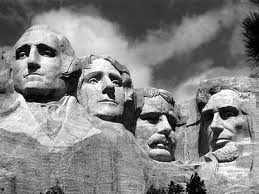
\includegraphics[width=3.6in]{Images/MtRush.png}

Here we have only one image, and we'll use NMF to compress it, not do
classification.  First obtain $A$:

\begin{lstlisting}
> library(pixmap) 
# read file
> mtr <- read.pnm('MtRush.pgm') 
> class(mtr)
[1] "pixmapGrey"
attr(,"package")
[1] "pixmap"
# mtr is an R S4 object of class "pixmapGrey"
# extract the pixels matrix
> a <- mtr@grey
\end{lstlisting}

Now, perform NMF, find the approximation to $A$, and display it:

\begin{lstlisting}
> aout <- nmf(a,50)
> w <- aout@fit@W
> h <- aout@fit@H
> approxa <- w %*% h
# brightness values must be in [0,1]
> approxa <- pmin(approxa,1) 
> mtrnew <- mtr
> mtrnew@grey <- approxa 
> plot(mtrnew) 
\end{lstlisting}

Here is the result:

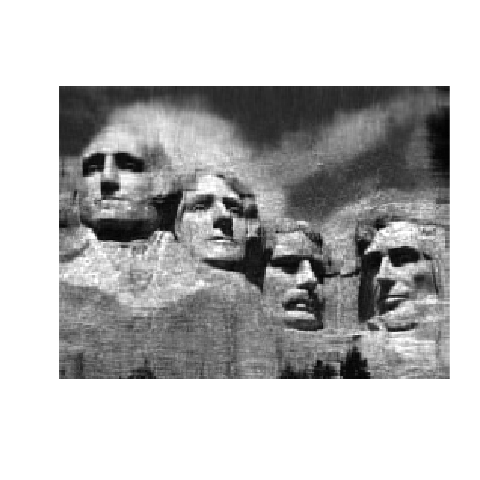
\includegraphics[width=3.6in]{Images/MtRush50.png}

This is somewhat blurry.  The original matrix has dimension $194 \times
259$, and thus presumably has rank 194.\footnote{One could check this by
finding the number of nonzero eigenvalues of $A'A$, say by running
\textbf{prcomp()}.} We've approximated the matrix by one of rank only
50, a storage savings.  Not important for one small picture, but
possibly worthwhile if we have many. The approximation is not bad in
that light, and may be good enough for image recognition or other
applications.

\subsection{Computation}

How are the NMF solutions found?  What is {\bf nmf()} doing internally?

Needless to say, the methods are all iterative, with one approach being
that of the Alternating Least Squares algorithm.  It's quite intuitive,
builds on our previous material, is easily adapted to the RS setting,
and provides insight into NMF itself.

By the way, this is not the default for {\bf nmf()}.  To select it, set
{\bf method = 'snmf/r'}.

\subsubsection{Objective Function}

We need an {\it objective function}, a criterion to optimize, in this
case a criterion for goodness of approximation. Here we will take that
to be the {\it Frobenius} norm, which is just the Euclidean ($l_2$)
norm with the matrix treated as a vector:\footnote{The $l_p$ norm of a
vector $v = (v_1,...,v_r)$ is defined to be

$$
||v||_p = \left (\sum_i |v_i|^p \right )^{1/p}
$$
}

\begin{equation}
\label{froben}
\|Q\|_2 = 
\sqrt{
\sum_{i,j} Q_{ij}^2
}
\end{equation}

So our criterion for error of approximation will be

\begin{equation}
\label{errawh}
\|A - WH\|_2
\end{equation}

This measure is specified in {\bf nmf()} by setting {\bf objective =
'euclidean'}.

\subsubsection{Alternating Least Squares}

So, how does Alternating Least Squares work?  Suppose just for a moment
that we know the exact value of $W$, with $H$ unknown.  Then for each
$j$ we could minimize

\begin{equation}
\label{errajwhj}
\|A_{\cdot j} - W H_{\cdot j}\|_2
\end{equation}

We are seeking to find $H_{\cdot j}$ that minimizes (\ref{froben}), with
$A_{\cdot j}$ and $W$ known.  But since the Frobenius norm is just a sum
of squares, that minimization is just a least-squares problem, i.e.\
linear regression!  We are ``predicting'' $A_{\cdot j}$ from $W$,

In the notation of Section \ref{lmdetails}:

\begin{itemize}

\item The matrix $A$ there is our $W$ here, known.

\item The vector $D$ there is our $A_{\cdot j}$ here, known.

\item The vector $b$ there is our $H_{\cdot j}$ here, unknown and to be
solved for.

\end{itemize} 

There is one difference, though.  Recall that $A$ in Section
\ref{lmdetails} included a column of 1s, to accommodate the $\beta_0$
term in the model.  We don't have that here, so we need to tell
\textbf{lm()} to omit it.  We compute 

\begin{lstlisting}
> h[,j] <- lm(a[,j] ~ w - 1)
\end{lstlisting}

for each $j$.\footnote{The -1 specifies that we do not want a constant term in
the model.}

On the other hand, suppose we know $H$ but not $W$.  We could take 
transposes,

\begin{equation}
A' = H' W'
\end{equation}

and then just interchange the roles of $W$ and $H$ above.  Here a call
to {\bf lm()} gives us a row of $W$, and we do this for all rows.

Putting all this together, we first choose initial guesses, say random
numbers, for $W$ and $H$; {\bf nmf()} gives us various choices as to how
to do this.  Then we alternate: Compute the new guess for $W$ assuming
$H$ is correct, then choose the new guess for $H$ based on that new $W$,
and so on.

During the above process, we may generate some negative values.  If so,
we simply truncate to 0.

\subsubsection{Dealing with the Missing Values}

In our RS setting, of course, most of $A$ is missing.  But we can easily
adapt to that.  In (\ref{errajwhj}), simply replace $A_{\cdot j}$ by the
known elements of that vector, and replace $W$ by the corresponding
rows.  Then proceed as before.

% \subsubsection{Multiplicative Update}
% 
% Alternating Least Squares is appealing in several senses.  At each
% iteration, it is minimizing a {\it convex} function, meaning in essence
% that there is a unique local and global minimum; it is easy to
% implement, since there are many least-squares routines publicly
% available, such as {\bf lm()} here; and above all, it has a nice
% interpretation, predicting columns of $A$.
% 
% Another popular algorithm is {\it multiplicative update}, due to Lee and
% Seung.  Here are the update formulas for $W$ given $H$ and {\it vice
% versa}:
% 
% \begin{equation}
% W \leftarrow W \circ 
% \frac
% {AH'}
% {WHH'}
% \end{equation}
% 
% \begin{equation}
% H \leftarrow H \circ 
% \frac
% {W'A}
% {W'WH}
% \end{equation}
% 
% where $Q \circ R$ and $\frac{Q}{R}$ represent \underline{elementwise}
% multiplication and division with conformable matrices $Q$ and $R$, and
% the juxtaposition $QR$ means ordinary matrix multiplication.

\subsubsection{Convergence and Uniqueness Issues}

There are no panaceas for applications considered here.  Every solution
has potential problems.

With NMF, one issue is uniqueness --- there might not be a unique pair
$(W,H)$ that minimizes (\ref{errawh}).\footnote{See Donoho and
Stodden,{\it When Does Non-Negative Matrix Factorization Give a Correct
Decomposition into Parts?},
\url{https://web.stanford.edu/~vcs/papers/NMFCDP.pdf}.}  In fact, one
can see this immediately:  Doubling $W$ while having $H$ leaves the
product $WH$ unchanged.  Of course, the product is all that really
counts, but in turn, this may result in convergence problems. The NMF
documentation recommends running {\bf nmf()} multiple times; it will use
a different seed for the random initial values each time.

The Alternating Least Squares method used here is considered by some to
have better convergence properties, since the solution at each iteration
is unique.  This may come at the expense of slower convergence.

\subsection{Predicting New Cases}

How do we find $q$, the coordinates of a new user, using her ratings
record $u$?  The answer is that again we can use the least-squares idea
above.

\begin{lstlisting}
> q <- lm(u ~ h - 1)
\end{lstlisting}

\subsection{How Do We Choose the Rank?}

This is not an easy question.  One approach would be to use
\textbf{prcomp}, or for that matter \textbf{svd()}, to find the
eigenvalues, then take our rank to be the number of ``large''
eigenvalues, as discussed in Chapter \ref{chap:linalg}.  

Of course, the typical way rank is chosen is cross validation.

\subsection{Why Nonnegative?}

In the applications we've mentioned here, we always have $A_{ij} \geq 0$.
However, that doesn't necesarily mean that we need $W$ and $H$ to be
nonnegative, since we could always truncate to 0 in the product
$WH$.\footnote{Indeed, we probably want to truncate at the high end too.
If say the maximum possible rating is 5, we would truncate any
prediction higher than that.}

There are a couple of reasons NMF may be preferable.  First, truncation
may be questionable if we have a lot of negative values.  But the second
reason is that NMF may be more useful, as follows:

In a facial image recognition case, say, there is hope that the vectors
$W_{\cdot j}$ will be {\it sparse}, i.e.\ mostly 0s. Then we might have,
say, the nonzero elements of $W_{\cdot 1}$ correspond to eyes, $W_{\cdot
2}$ correspond to nose and so on with other parts of the face.  We are
then ``summing'' to form a complete face.  This may enable effective
{\it parts-based recognition}, with helpful interpretations.

In our RS setting, this parts-based effect, NMF would give us crisper
distinction among the various synthetic users.  This may reveal clusters
of user behavior, which could be quite helpful to the analyst.

\section{Functions in rectools}

The \textbf{rectools} package implements NMF via the \textbf{recoSystem}
by Chih-Jen Li \textit{et al}, providing wrappers to \textbf{recoSystem}
functions.  Basic call forms are:

\begin{lstlisting}
trainReco(ratingsIn,rnk=10,nmf=FALSE)
predict.RecoS3(recoObj,testSet)
\end{lstlisting}

Here \textbf{ratingsIn} is the usual three-column (userID,itemID,rating)
(plus covariates, if any) data frame; \textbf{rnk} is the desired rank;
\textbf{nmf} is false for SVD, true for NMF; \textbf{recoObj} is the 
return value from \textbf{trainReco()}; and \textbf{testSet} is the test
set, in the same format as \textbf{ratingsIn}, minus the ratings column.

The return value from \textbf{trainReco()} is an R S3 object of class
'RecoS3', with components $P$ and $Q$, corresponding to $W$ and $H'$ in
our notation.  In the case of covariates (see below), some R
\textbf{attributes} are also included.

\section{Dealing with Covariates}

The easiest approach to handling covariates is to simply ``subtract them
out'' for the data via linear regression, then run NMF/SVD on the resulting
\textit{residuals}, and finally, at the prediction stage, add the
regression values back in.

Here are relevant code excerpts:

\textbf{trainReco()}:

\begin{lstlisting}
hasCovs <- (ncol(ratingsIn) > 3)
if (hasCovs) {
    covs <- as.matrix(ratingsIn[, -(1:3)])
    lmout <- lm(ratingsIn[, 3] ~ covs)
    minResid <- min(lmout$residuals)
    ratingsIn[, 3] <- lmout$residuals - minResid
}
...
r$train(train_set, opts = list(dim = rnk, nmf = nmf))
result <- r$output(out_memory(), out_memory())
attr(result, "hasCovs") <- hasCovs
if (hasCovs) {
    attr(result, "covCoefs") <- coef(lmout)
    attr(result, "minResid") <- minResid
}
class(result) <- "RecoS3"
result
\end{lstlisting}

\textbf{predict.RecoS3()}:

\begin{lstlisting}
if (hasCovs) {
     tmp <- c(1, testCovs[i, ]) %*% covCoefs + minResid
}
pred[i] <- p[j, ] %*% q[k, ] + tmp
\end{lstlisting}

The return value from \textbf{lm()} includes a \textbf{residuals}
component, equal to the difference between the actual ``Y'' value and
the fitted estimated regression function.  In the covariates case, 
\textbf{trainReco()} replaces the ratings by the residuals, so the
product $WH$ approximates them rather than the original $A$.

Then in \textbf{predict.RecoS3()}, after multiplying $W_{i \cdot}$ and
$H_{\cdot j}$, the estimated regression function value for the given
case is added back in.

The role of \textbf{minResid} is this:  If we are using NMF, fitting to the
residuals, which are both positive and negative, makes no sense.  So, we
subtract the (algebraically) smallest residual, resulting in only
nonnegative values.  Again, this is added back in later on.

\section{Regularization}

In recent years, there has been much interest in \textit{regularizing}
statistical estimates of various kinds.  In regression analysis, for
instance, the idea is to shrink the $\widehat{\beta}$ vector somewhat.
There is some theoretical foundation for this, and it is viewed by many
as especially useful for dimension reduction.

In the notation of Chapter \ref{chap:infra2}, instead of choosing $b$ to
minimize

\begin{equation}
||D - Ab|||_2
\end{equation}

we minimize

\begin{equation}
\label{ridge}
||D - Ab||_2 + \gamma ||b||_2
\end{equation}

or

\begin{equation}
\label{lasso}
||D - Ab||_2 + \gamma ||b||_1
\end{equation}

Here $\gamma$ is a hyperparameter, as usual chosen via cross validation.
This parameter acts as a ``governmor,'' preventing the minimizing $b$
from becoming too large.  The methods based on (\ref{ridge}) and
(\ref{lasso}) are called \textit{ridge regression} and the
\textit{LASSO}, respectively.

The LASSO is especially popular because it can be used as a variable
selection procedure.  Typically the minimizing $b$ will have many or
most of its components equal to 0, essentially eliminating the
corresponding predictors.

For NMF (or SVD), we probably don't want to force some predicted ratings
to 0, so ridge is the better choice.  Thus, instead of choosing $W$ and
$H$ to minimize (\ref{errawh}), we minimize

\begin{equation}
||A - WH||_2 + \gamma_1 ||W||_2^2 + \gamma_2 ||H||_2^2
\end{equation}

(typically the squared norms are used rather than the norms themselves).

\section{``Bias'' Removal}

As noted in Chapter \ref{chap:knn}, some users tend to give more liberal
ratings, while others tend to be more cautious.  Similarly, some items
tend to be rated more highly than others.  One way of dealing with
that is to adjust our ratings matrix $A$ accordingly:  For each user
$i$, let $R_i$ denote the average of all known ratings from that user.
Also, for each item $j$ let $S_j$ denote the average of all known ratings
for that item.  These are termed \textit{biases}. Then do the replacement

\begin{equation}
A_{uv} \leftarrow A_{uv} - R_u - S_v
\end{equation}

and then form the matrix factorization as usual.  In the end, after
estimating the unknown entries in $A$, restore
the subtracted quantities:

\begin{equation}
A_{uv} \leftarrow A_{uv} + R_u + S_v
\end{equation}
